\subsection{Spiking Neural Networkの構成}

Spiking Neural Network (SNN) は前述した通り, 脳神経回路におけるパルス信号を介した情報処理を模倣したニューラルネットワークである\cite{generalsnn}.
そのため, 通常のArtificial Neural Network (ANN) と比較して, より生物学的妥当性が高いモデルとされている.
SNNはパルス状の電気信号を, スパイクと呼ばれる0か1の値を持つ信号として扱う.
さらに, スパイクが時間軸に沿って並べられたものをスパイク列と呼び, SNNはこのスパイク列をニューロン間で伝達することで, ニューロンの時間的なダイナミクスを模倣し情報処理を行う.

SNNの第$l$層における入出力の流れを\figref{fig:snn:inoutflow}に示す.
まず, 第$l$層へ入力されたスパイク$\bm{o}^{t, l-1}$は\eqrefc{eq:input_spike}によって重み付けされシナプス電流$\bm{i}^{t,l}$へ変換される.

\begin{equation}
    \bm{i}^{t, l} = \bm{W}^l\bm{o}^{t, l-1} + \bm{b}^l
    \label{eq:input_spike}
\end{equation}
ここで, $t$はその時刻を表し, $\bm{W}^l, \bm{b}^l$はそれぞれ第$l$層のニューラルネットワークの重みとバイアスを表す.

次に, 第$l$層のSNNの内部状態$\bm{v}^{t, l}$は, 神経細胞活動の数理モデルによって更新される.
本研究では, 数理モデルとしてLeaky Integrate-and-Fire (LIF) モデル (\eqrefc{eq:lif}) を用いる.
LIFモデルでは, 入力シナプス電流$\bm{i}^{t, l}$を, 神経細胞の内部状態$\bm{v}^{t, l}$があるしきい値に達するまで時間的な積分を行う.

\begin{equation}
    {\tau}\frac{d\bm{v}^l}{dt}=-\left(\bm{v}^{t-1,l}-v_{rest}\right)+r\bm{i}^{t, l}
    \label{eq:lif}
\end{equation}
ここで, $\tau$は神経細胞の時定数, $v_{rest}$は内部状態の初期状態, $r$は神経細胞の膜抵抗である.

最後に, 内部状態$\bm{v}^{t, l}$が一定の閾値$v_{th}$を超えたときに出力スパイク$\bm{o}^{t, l}$が1となって出力される (\eqrefc{eq:outputSpike1:1}, \eqrefc{eq:outputSpike1:2}).
また, 閾値を超えた内部状態は初期状態へとリセットされる (\eqrefc{eq:outputSpike2:1}, \eqrefc{eq:outputSpike2:2}).

\begin{equation}
  \bm{o}^{t, l}=g\left(\bm{v}^{t, l}\right) \label{eq:outputSpike1:1}
\end{equation}
\begin{equation}
  \begin{split}
    \text{where} \hspace{3cm}\ \\
    g\left(x\right)=\left\{
      \begin{alignedat}{2}
        1 &\:\left(x{\geq}v_{th}\right)\\
        0 &\:\left(x{<}v_{th}\right)
      \end{alignedat}
    \right. \label{eq:outputSpike1:2}
  \end{split}
\end{equation}

\begin{equation}
  \bm{v}^{t, l}=h\left(\bm{v}^{t, l}\right)
  \label{eq:outputSpike2:1}
\end{equation}
\begin{equation}
  \begin{split}
    \text{where} \hspace{3cm}\ \\
    h\left(x\right)=\left\{
      \begin{alignedat}{2}
        &v_{rset} &\:\left(x{\geq}v_{th}\right)\\
        &x &\:\left(x{<}v_{th}\right)
      \end{alignedat}
  \right. 
  \end{split} \label{eq:outputSpike2:2}
\end{equation}


\begin{figure}[htb]
    \centering
    % \includesvg[width=0.9\textwidth, inkscapelatex=false]{Static/chap2_sec1_snn}
    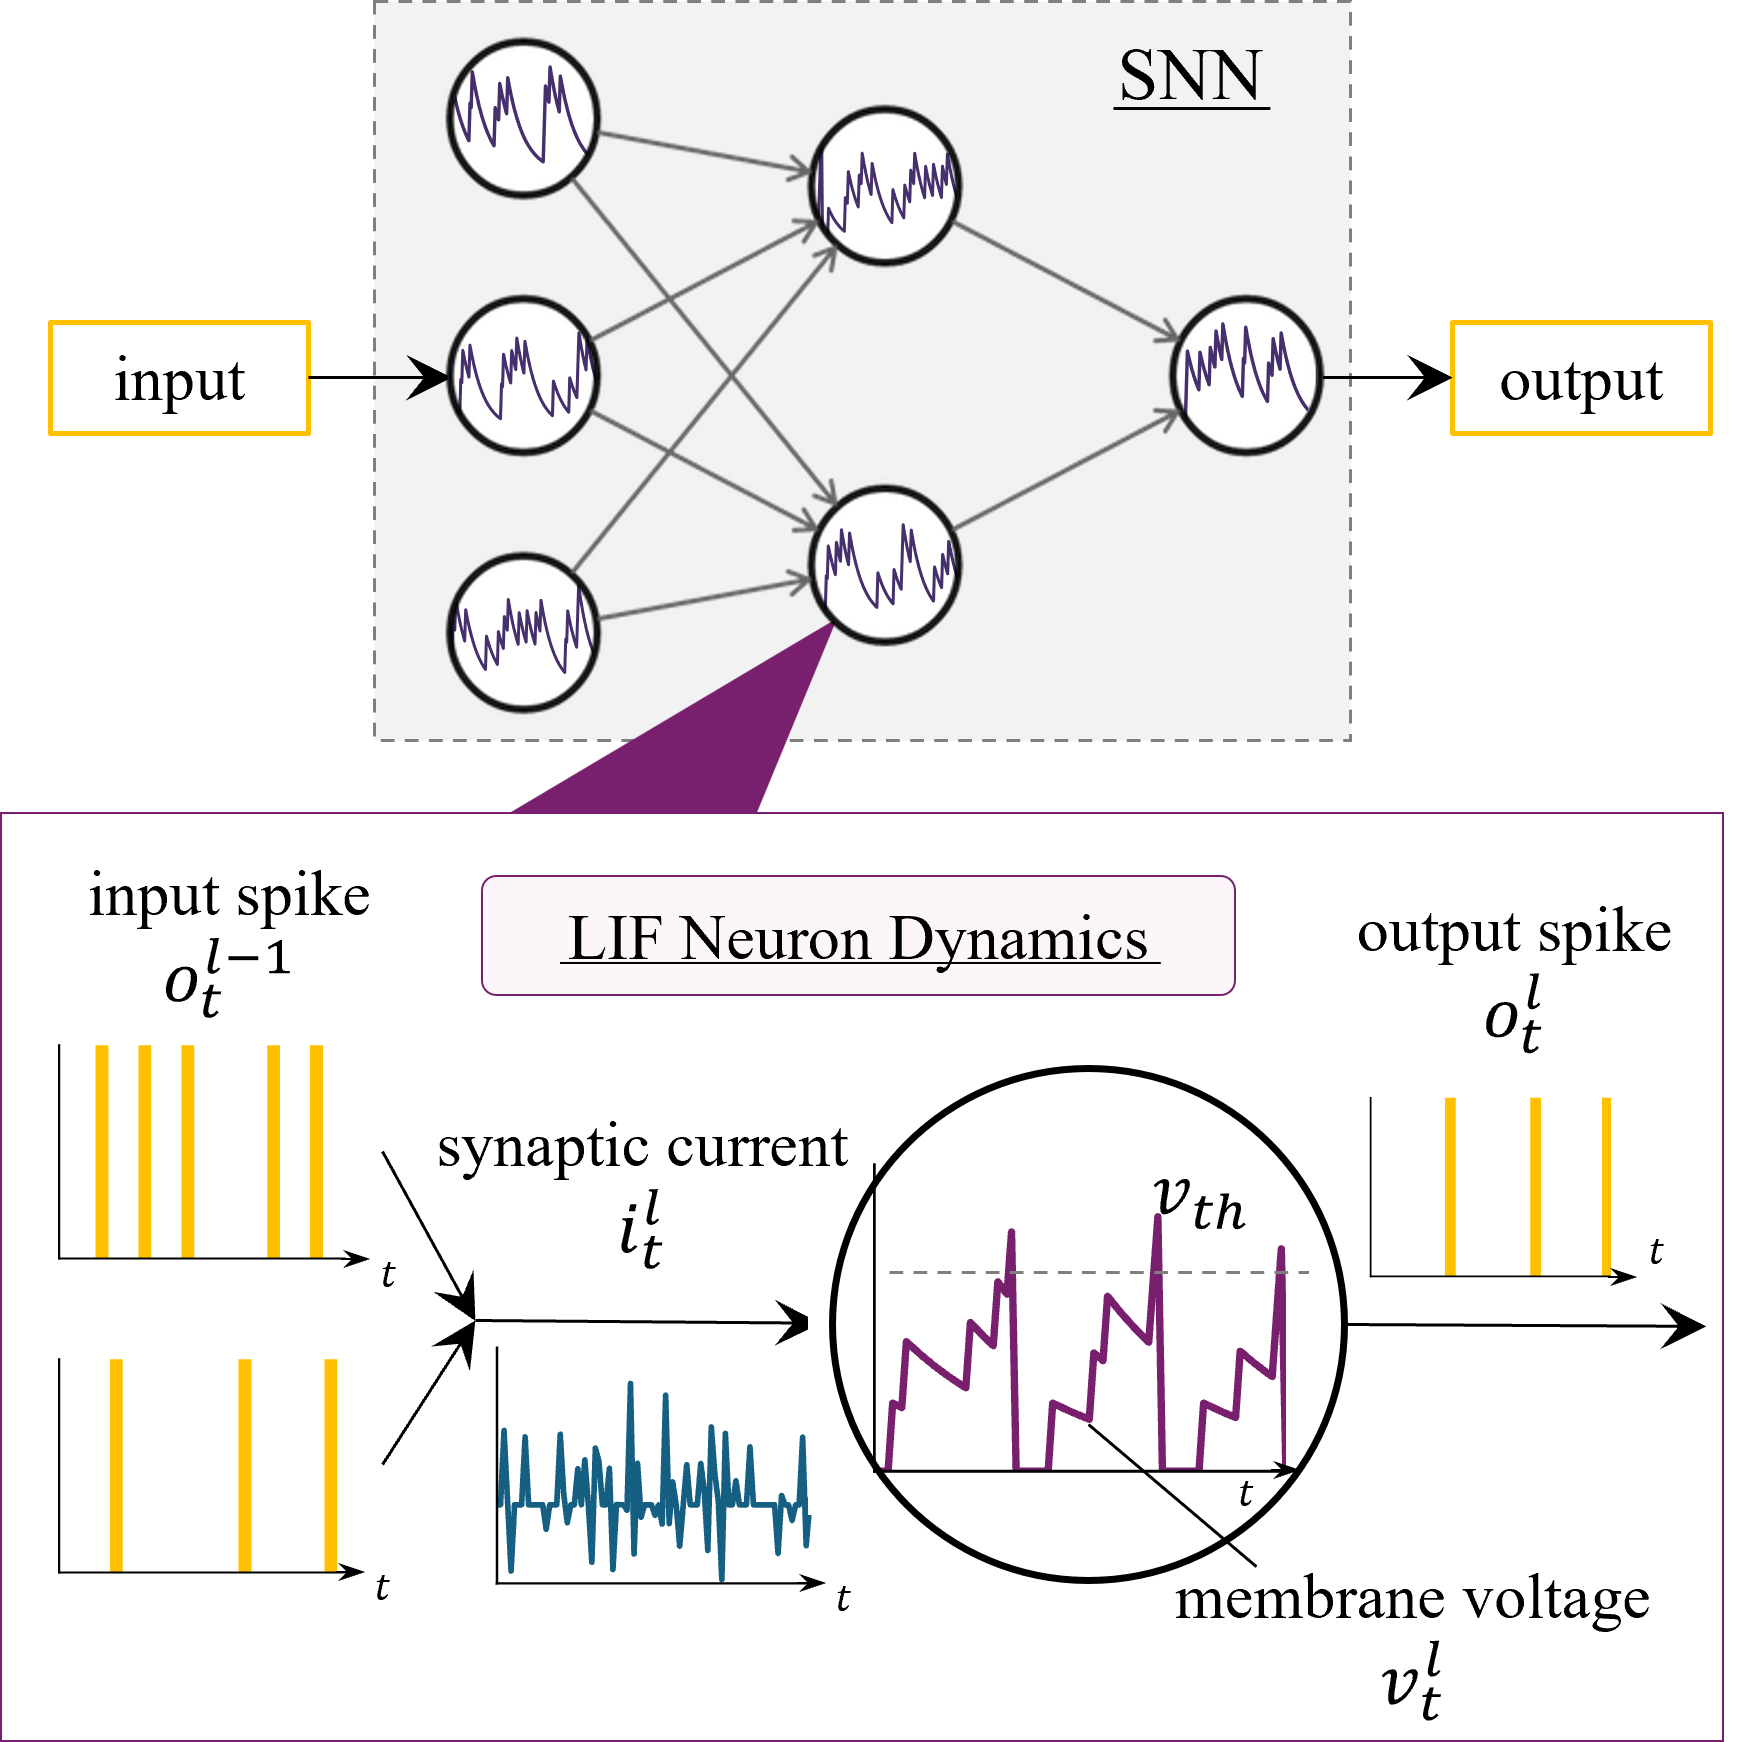
\includegraphics[width=0.75\textwidth]{Static/chap2_sec1_snn.png}
    \caption{SNNの入出力の流れ}
    \label{fig:snn:inoutflow}
\end{figure}

一般的に, ANNの学習には誤差逆伝播法が用いられる.
誤差逆伝播法とは, ニューラルネットワークの出力と学習データの損失の勾配を用いて, ネットワークの各パラメータを更新する手法である.
本研究では, 誤差逆伝播法をSNNの学習に拡張したSpatio-Temporal Backpropagation (STBP)則\cite{stbp}を用いる.
